\documentclass[a4paper]{scrreprt}
\usepackage{fancyhdr}
\pagestyle{fancy}
\usepackage[english]{babel}
\usepackage[utf8]{inputenc}
\usepackage{graphicx}
\usepackage{url}
\usepackage{textcomp}
\usepackage{amsmath}
\usepackage{lastpage}
\usepackage{pgf}
\usepackage{wrapfig}
\usepackage{fancyvrb}
\usepackage{pdfpages}

\usepackage{etoolbox}
\makeatletter
\patchcmd{\scr@startchapter}{\if@openright\cleardoublepage\else\clearpage\fi}{}{}{}
\makeatother

\newcommand{\code}[1]{\texttt{#1}}

% Create header and footer
\headheight 27pt
\pagestyle{fancyplain}
\lhead{\footnotesize{Applikationer för internet, ID1354}}
\chead{\footnotesize{Assignment 2 report}}
\rhead{}
\lfoot{}
\cfoot{\thepage\ (\pageref{LastPage})}
\rfoot{}

% Create title page
\title{Assignment 2}
\subtitle{Applikationer för internet, ID1354}
\author{Max Körlinge, korlinge@kth.se}
\date{\today}

\begin{document}

\maketitle

\tableofcontents %Generates the TOC
\clearpage

\chapter{Introduction}

This assignment concerns working on the PHP server to implement user authentication, users being able to write comments on recipes, and users being able to delete those comments. Optional tasks were being able to register new users on the site, and storing all recipe data in XML format. I chose to do all tasks (optional and mandatory).

\chapter{Literature Study}

To complete the task I first studied the course lecture notes on the PHP language, PHP for the web server, and XML.

\chapter{Method}

\section{Task 1}

To implement authentication I created a new login page with a form that submits to a php script. The script uses PDO to make a connection to the mySQL database I setup to check wheither there is a matching username - password entry in the database. I use the \code{$_SESSION} variable to store the username and implemented a check in the header included in every page if the user is logged in or not. To clarify for the user that there is loading going on a redirection page was implemented, telling the user what is happening.

\section{Task 2}

The commenting functionality was implemented by including a form at the bottom of the page if the user is logged in (by using the function developed for task 1). The form submits using a PHP script that uses the \code{$_POST} and \code{$_SESSION} variables to find the comment submitted and the username submitting it, and uses a PDO connection to the mySQL database to store it. While developing this it was also necessery to rework the recipe sites to load comments from the database, instead of hardcoding them as before.

\section{Task 3}

I used the method described in the lecture notes on using hidden input fields in forms to implement being able to delete a comment. The hidden value field is given the recipe_id stored in the mySQL database, and then the form submits a script which simply querys the database to delete this entry. While generating the list of comments to the page from the database, the program checks wheither the processed comment was written by the currently logged in user, and then places the delete form next to that comment. No delete button is shown for comments that are not written by the currently logged in user.

\section{Optional Task 1}

To register new users I added a new page for registrations which is very similar to the login page, to keep the design coherent. It uses a similar method to the login page: submitting a form to a PHP script, and the PHP script extracting the new username and password, checking the database for wheither this username already exists (if so returning to the registration page), and if it does not, adding the username and password to the database. The user is then able to log in with the new account.

\section{Optional Task 2}

To store the recipes in XML I used the provided mycookbook template to convert my recipes stored in HTML to properly matching XML tags for this template. I chose to put all recipes in the same xml file, to preserve an order which also could be used to find a matching recipe ID for the database. For example, the first recipe in the XML file has recipe_id 1 in the database. I used SimpleXML to parse the XML, and rewrote the recipe sites to call a PHP file called recipe.php with a function \code{RecipeSite($name)} where you can input the name of a recipe in the database, and it will be output the contents correctly to the site.


-TODO
\chapter{Result}
\label{sec:result}

\section{Task 2}

The git repository can be found at https://github.com/fongie/TastyRecipes/tree/assignment2
The site contains the parts specified in the assignment: a welcoming home page (Fig. \ref{fig:design}), a calendar page with two recipes, and a page each for the recipes themselves.

\begin{figure}[h!]
  \begin{center}
    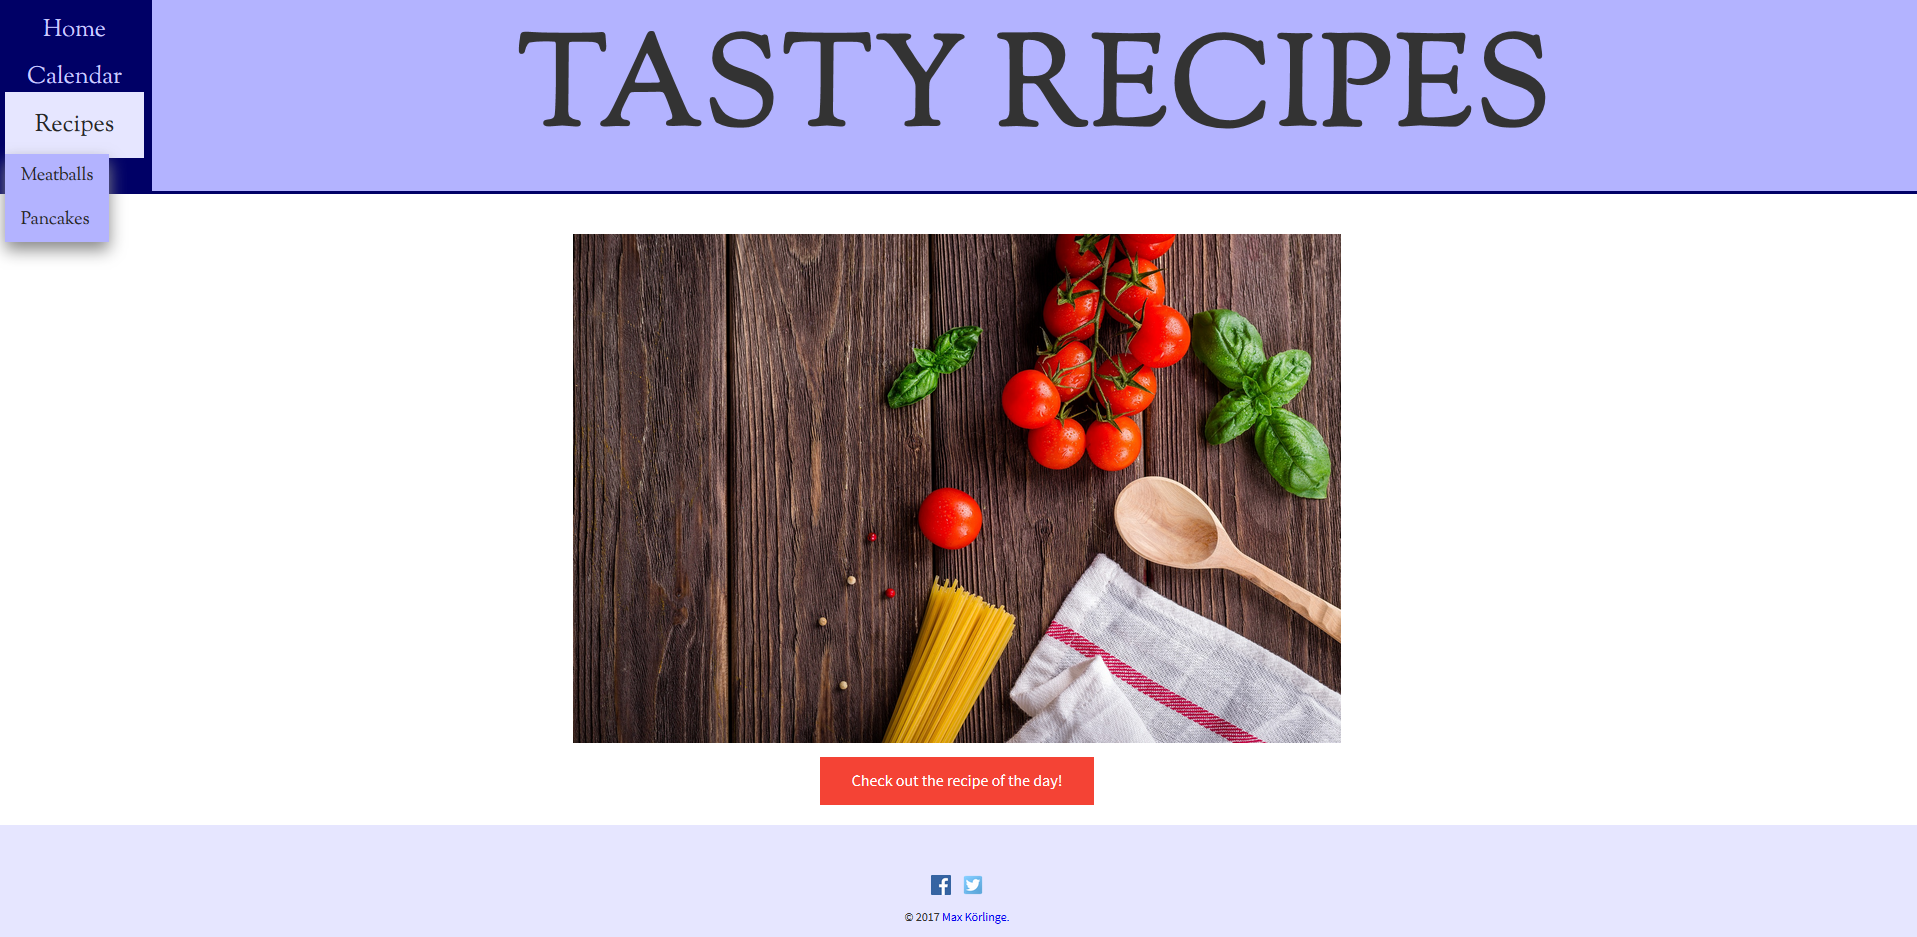
\includegraphics[scale=0.41]{design.png}
    \caption{The index page, showing navbar hover.}
    \label{fig:design}
  \end{center}
\end{figure}

All files passed the W3C validation, as shown in Figure \ref{fig:htmlvalidations} and \ref{fig:cssvalidations}. The files were also tested individually, as opposed to providing just the URL.

\begin{figure}[h!]
  \begin{center}
    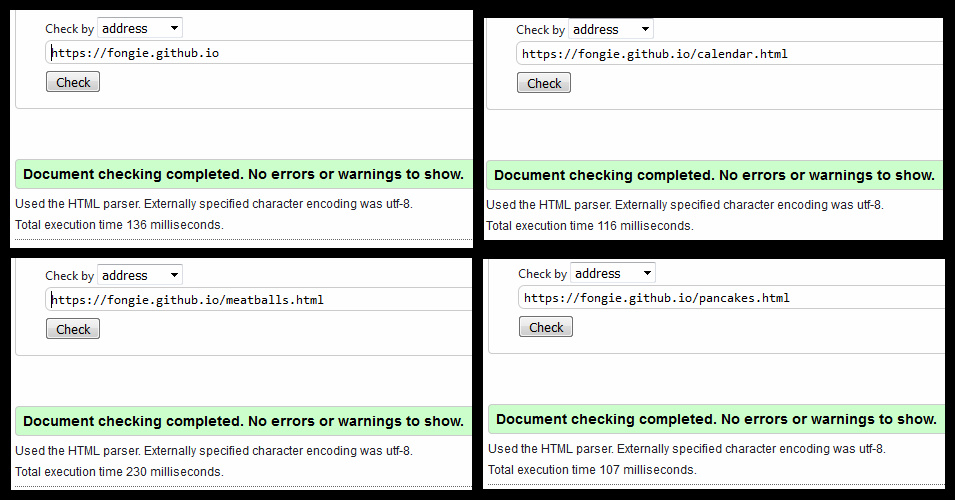
\includegraphics[scale=0.41]{htmlval/html_checks.jpeg}
    \caption{All W3C html validations.}
    \label{fig:htmlvalidations}
  \end{center}
\end{figure}

\begin{figure}[h!]
  \begin{center}
    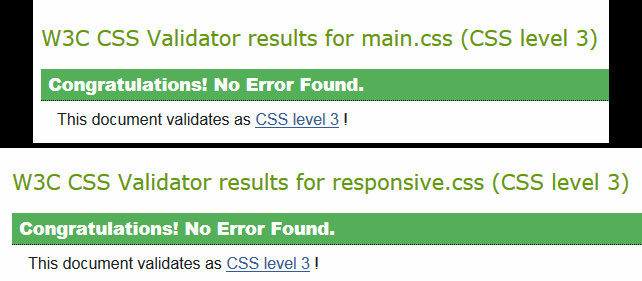
\includegraphics[scale=0.41]{cssval/css_checks.jpeg}
    \caption{All W3C css validations.}
    \label{fig:cssvalidations}
  \end{center}
\end{figure}


\section{Task 3}

Visibility of system status was considered but not found applicable for the site. Currently the site is completely static and does not have anything going on other than moving between static pages, so no loading or new elements appearing on the same site, and thus there is no real system status that needs to be shown to the user. Later I imagine there will be, when user will be able to post comments for example, the user would need to be told if the comment is being posted, failed to be posted, or was successfully posted.

A match between system and real world was sought after by not using any technical terms. The index page is called "Home", and in general there are normal, non-technical, words used throughout the site.

When it comes to consistency and standards the layout is fairly conventional as the navigation can be found somewhere at the top and in a bar of some sort. Also, all links are clearly displayed as buttons or images and the "pointer" cursor is used when hovering over links.

Recognition rather than recall is maintained mainly by the navbar, since all pages are always accessible through the navbar there is no need for the user to memorize how they got somewhere on the site.

The design is aestethic and minimalistic, using a sparse color palette of white and blue with only one alert-type red button. There is no eccess images or text floating about that do not add to the content or usability of the site. You are always only one or two clicks away from a recipe, and when arriving at the recipe you only have a picture of the food and bulleted lists of ingredients and how to make it.

\section{Task 4}

Although I unfortunately could not test Safari 9 I did test the others and it appears to be the same. I chose to display the Calendar page here since I think it might be the one that has the most complex css that could prevent compatibility, see Figure \ref{fig:compcheck}. Since I used different tools it was not possible to get them all at the same resolutions, but it is clear that they appear the same in all browsers nevertheless.

\begin{figure}[h!]
  \begin{center}
    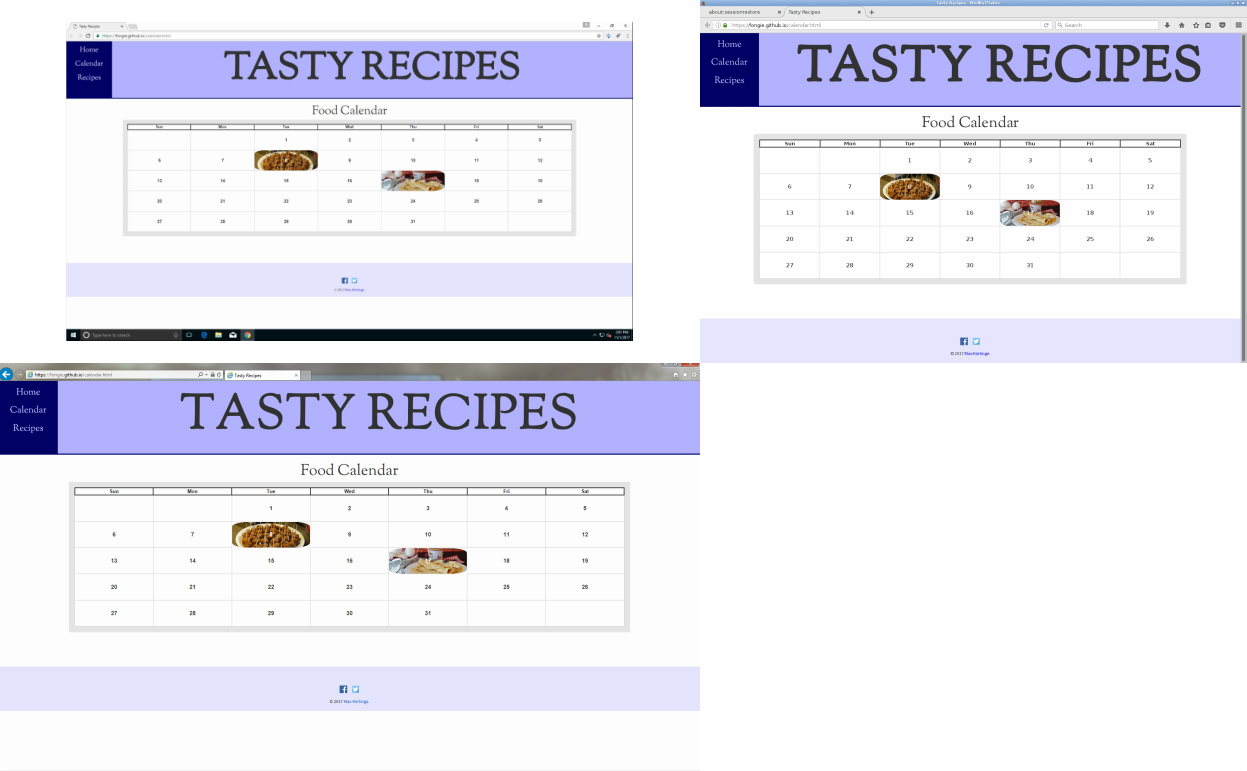
\includegraphics[scale=0.41]{compatability_check.jpg}
    \caption{Top left: Chrome 55, Top Right: Firefox 50, Bottom left: IE 10}
    \label{fig:compcheck}
  \end{center}
\end{figure}

\section{Optional Task 1}

The site was actually first designed for small resolution and later expanded to larger resolutions, by for example making some fonts larger, some images take less proportion of the screen, and moving the navbar to the left of the header. You can see the full size in Figure \ref{fig:design}, and the mobile version in Figure \ref{fig:mobversion}.

\begin{figure}[h!]
  \begin{center}
    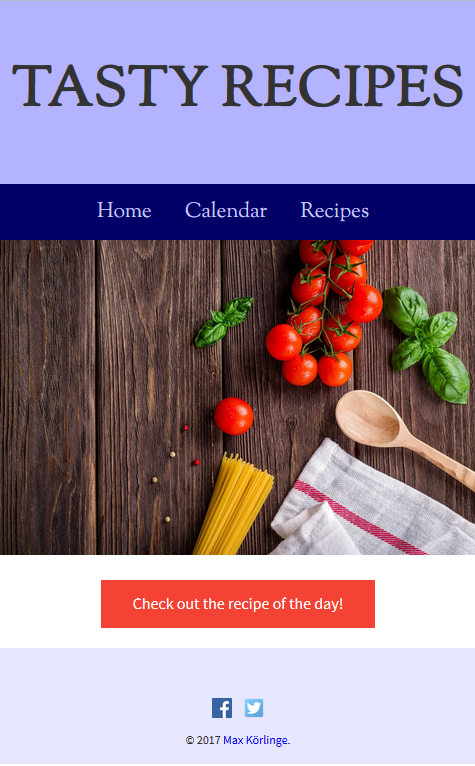
\includegraphics[scale=0.41]{mobversion.png}
    \caption{The mobile version.}
    \label{fig:mobversion}
  \end{center}
\end{figure}

\section{Optional Task 2}

The site has alt texts for all images and does not rely on color for example for highlighting things. When hovering over the calendar for example, it does not show where you are by changing color, but instead by giving the current cell a shadow which makes the cell "pop". As shown above all HTML and CSS was validated and thus used properly, and also as discussed previously, the navbar provides clear navigation mechanisms by always being present at a predictable place, and having links to all available pages.

\chapter{Discussion}

kom ihåg att påpeka att receptsidorna kunde vara mer dynamiskt genererade, men att det uppfyller kraven


\chapter{Comments About the Course}

This is a fun and practical assignment. I found the required browsers to check really hard to find on any online tool, which was a little frustrating.

I spent about 15 hours on this assignment.


\end{document}
